% Chapter 2

\chapter{Methodology and approach} % Write in your own chapter title
\label{Chapter2}

We have implemented our pipeline in C and on Linux platform, so that it
can easily be ported from a PC to embedded environment. Wherever
possible, we have used opencv library to carry intended job. Our top
level pipeline can be explained as in figure ~\ref{image_pipeline}.
\begin{figure}[!b]
\centering
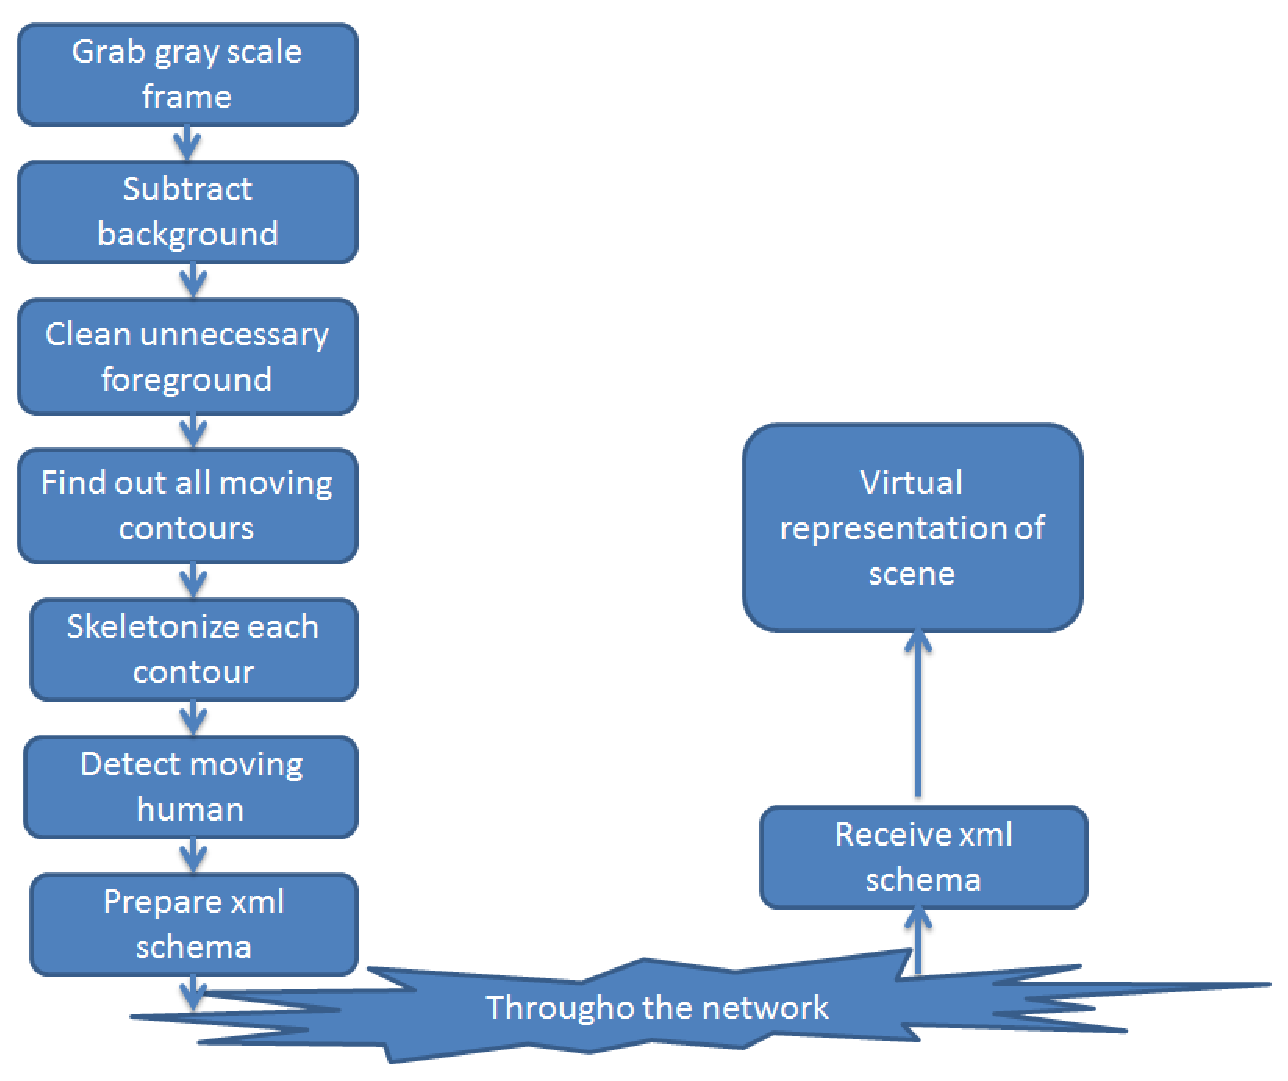
\includegraphics[scale=0.60]{Figures/image_pipeline}
\caption{Low BW surveillance Image Pipeline}
\label{image_pipeline}
\end{figure}


Since background subtraction has key role in accomplishing intended job,
therefore we have compared two recently developed efficient background
subtraction algorithm and then choosed one of them in our final
work.First one ~\cite{11} is based on use of texture features present in
Local Binary Pattern(LBP). LBP works well with local illumination
changes, however there can be issues in case of global illumination
change.Author of this paper has done several improvements by using
photometric invariant color measurement and flexible weight updating for
background modes. However, computationally it is not so efficient
compared to second one ~\cite{9} which we have also selected for our
uses.  It is based on unique way of replacing background pixel value
over the time.It replaces background values for last N frames
randomly.Furthermore, it diffuses updated values to neighbouring pixels,
and again that too on random basis. So far selected algorithm surpasses
other existing algorithm in computation complexities. Figure
\ref{bg_compare} shows the comparison of execution time of these two
algorithm.

\begin{figure}[!b]
\centering
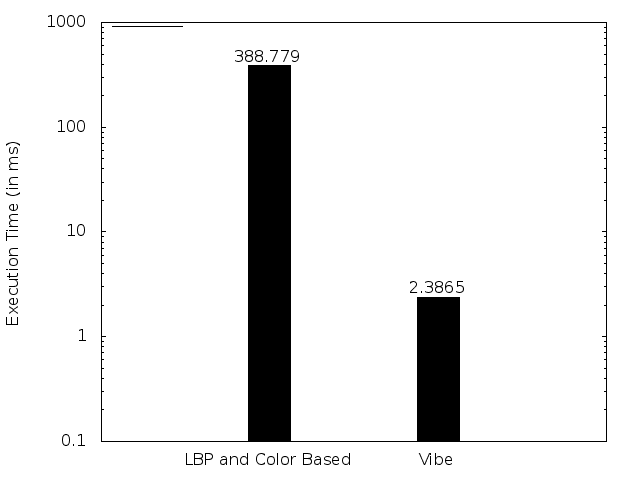
\includegraphics[scale=0.60]{Figures/bg_compare}
\caption{Variation of background subtraction execution time of ~\cite{11}
and ~\cite{9} with frame number. This timing was observed with a system
having having DMIPS = 800.}
\label{bg_compare}
\end{figure}

None of the background subtraction algorithm allows pure foreground
extraction. There would always be several noise object in the extracted
image. These are cleaned by morphological erosion operation followed by
dilation operation.Further all moving contours are separated out by
using opencv library ~\cite{34} function cvFindContours.This function
gives us boundary point of moving object.

Star skeletonization method has been used to find extreme point on
moving contours. This method plots distance of each boundary point from
the centroid and then uses peaks of the curve as skeleton
point.Following steps have been used to identify types of each moving
contours.
\begin{enumerate}
\item Centroid of each object is found out using following formula.\\
	\begin{equation}
	C_x = {1 \over N} \Sigma ^N _{i = 1} X_i 
	\end{equation}
	\begin{equation}
	C_y = {1 \over N} \Sigma ^N _{i = 1} Y_i 
	\end{equation}
Here X$_i$ and Y$_i$ are (X,Y) co-ordinate of i$_{th}$ point on the contour
boundary.
\item Distance d$_i$ is calculated between centroid and each boundary
point as follows.This calculated distance vector are stored in a CvMat
array.
	\begin{equation}
	d_i = \sqrt{(C_x - X_i)^2 + (C_y - Y_i)^2}
	\end{equation}

\begin{figure}[!b]
\centering
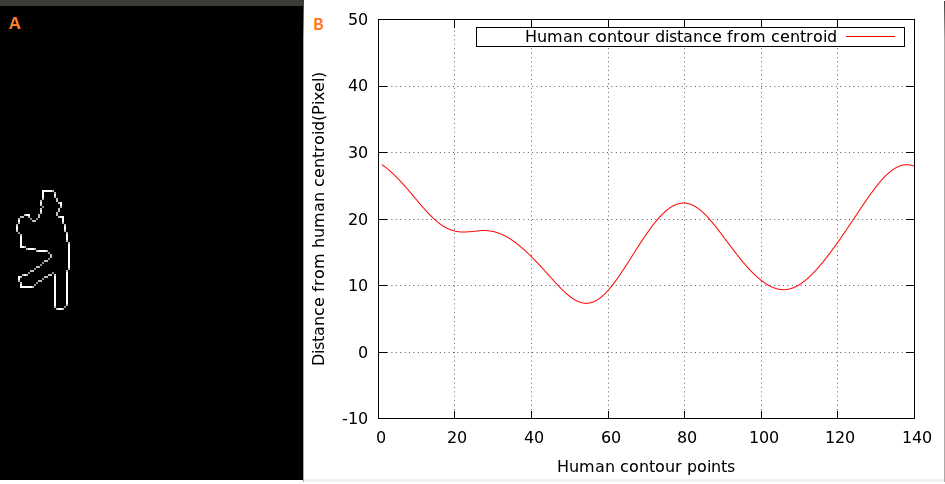
\includegraphics[scale=0.60]{Figures/distance}
\caption{Distance plot of human contour points from its centroid}
\label{distance}
\end{figure}

\item Distance vector array is smoothed to remove noise peaks using
cvSmooth.If these distances are plotted then it looks like fig
\ref{distance}. Now local maxima of distance vector is
calculated by finding zero crossing of difference vectors.\\ However,
even after smoothing operation there are some peaks which is not of our
interest.In our algorithm, we are using 2 most relevant peaks which are
nearest to each bottom corner of bounding box of contour respectively.
Only these two peaks along with centroid will give us sufficient information
to distinguish human among human, vehicle or animal etc.\\
In case of human these two peaks depicts two legs.For vehicle these are
just two extrema points of lower portion of back and front.In case of
animal these will correspond to front first leg and back last leg.
\item Let P$_1$(X$_1$, Y$_1$), P$_2$(X$_2$, Y$_2$) and C(C$_x$, C$_y$) are two peaks
nearest to bottom right and bottom left corner and centroid
respectively. Let $\theta$ is the angle between P$_1$C and P$_2$C, then
$\theta$ can be calculated as follows.\\
%
	\begin{equation}
	\theta = tan^{-1}[(Y_2 - C_y) / (X_2 - C_x)] \\ - tan^{-1}[(Y_1 - C_y) / (X_1 - C_x)]
	\end{equation}
%
If variation of this $\theta$ is plotted in respective frames for human
and vehicle then it looks like as shown in fig \ref{angle_plot}. There
are few points noticeable in the plot for human. First that, angle
variation pattern is repeatable. Second, It touches to 0 at some point.
For vehicle, it is almost constant as expected. We have not tried with a
video with animal. But, for animal there would be variation with
repeatable pattern but would never touch to zero.These criterion can be
the basis to identify about an object, whether it is a human, vehicle or
animal.

\begin{figure}[!b]
\centering
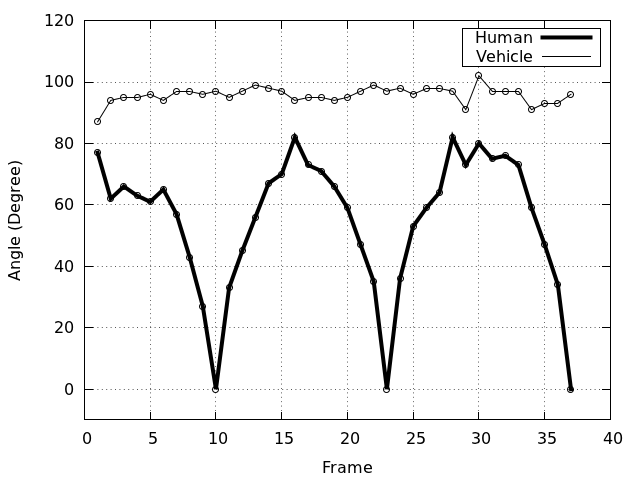
\includegraphics[scale=0.60]{Figures/angle_plot}
\caption{Variation of angle between legs with frame number for human and
vehicle.}
\label{angle_plot}
\end{figure}

\item We create a linked list of objects. When a new object comes in the
view of camera, a structure is created and added to the list.This new
object is tracked and value of (C$_x$, C$_y$), $\theta$ in each frame is
stored. 
\begin{enumerate} 
\item We track value of $\theta$ until it goes to '0' three times.
\item Now consider $\theta$ values between first and second '0' as
vector T$_1$ and $\theta$ values between second and third '0' as vector
T$_2$.
\item Find mean m$_1$ and m$_2$ of vector T$_1$ and T$_2$ respectively.
\item If n is the length of vector T$_1$ then calculate correlation value
between these two vectors to find similarities as follows.
	\begin{equation}
	corel = {{\Sigma ^n _{i = 1}(T_{1i} - m_1) * (T_{2i} - m_2)}
\over {\sqrt {\Sigma ^n _{i = 1} (T_{1i} - m_1)^2 * \Sigma ^n _{i = 1} (T_{2i}
- m_2)^2}}}
	\end{equation}
\item If correlation value is greater than a threshold value TH$_1$ then we say
that it is a human.

\end{enumerate} 
\end{enumerate}

